\documentclass[]{article}
\usepackage{lmodern}
\usepackage{amssymb,amsmath}
\usepackage{ifxetex,ifluatex}
\usepackage{fixltx2e} % provides \textsubscript
\ifnum 0\ifxetex 1\fi\ifluatex 1\fi=0 % if pdftex
  \usepackage[T1]{fontenc}
  \usepackage[utf8]{inputenc}
\else % if luatex or xelatex
  \ifxetex
    \usepackage{mathspec}
  \else
    \usepackage{fontspec}
  \fi
  \defaultfontfeatures{Ligatures=TeX,Scale=MatchLowercase}
\fi
% use upquote if available, for straight quotes in verbatim environments
\IfFileExists{upquote.sty}{\usepackage{upquote}}{}
% use microtype if available
\IfFileExists{microtype.sty}{%
\usepackage{microtype}
\UseMicrotypeSet[protrusion]{basicmath} % disable protrusion for tt fonts
}{}
\usepackage[margin=1in]{geometry}
\usepackage{hyperref}
\hypersetup{unicode=true,
            pdftitle={Lab: Decision Trees},
            pdfborder={0 0 0},
            breaklinks=true}
\urlstyle{same}  % don't use monospace font for urls
\usepackage{color}
\usepackage{fancyvrb}
\newcommand{\VerbBar}{|}
\newcommand{\VERB}{\Verb[commandchars=\\\{\}]}
\DefineVerbatimEnvironment{Highlighting}{Verbatim}{commandchars=\\\{\}}
% Add ',fontsize=\small' for more characters per line
\usepackage{framed}
\definecolor{shadecolor}{RGB}{248,248,248}
\newenvironment{Shaded}{\begin{snugshade}}{\end{snugshade}}
\newcommand{\KeywordTok}[1]{\textcolor[rgb]{0.13,0.29,0.53}{\textbf{#1}}}
\newcommand{\DataTypeTok}[1]{\textcolor[rgb]{0.13,0.29,0.53}{#1}}
\newcommand{\DecValTok}[1]{\textcolor[rgb]{0.00,0.00,0.81}{#1}}
\newcommand{\BaseNTok}[1]{\textcolor[rgb]{0.00,0.00,0.81}{#1}}
\newcommand{\FloatTok}[1]{\textcolor[rgb]{0.00,0.00,0.81}{#1}}
\newcommand{\ConstantTok}[1]{\textcolor[rgb]{0.00,0.00,0.00}{#1}}
\newcommand{\CharTok}[1]{\textcolor[rgb]{0.31,0.60,0.02}{#1}}
\newcommand{\SpecialCharTok}[1]{\textcolor[rgb]{0.00,0.00,0.00}{#1}}
\newcommand{\StringTok}[1]{\textcolor[rgb]{0.31,0.60,0.02}{#1}}
\newcommand{\VerbatimStringTok}[1]{\textcolor[rgb]{0.31,0.60,0.02}{#1}}
\newcommand{\SpecialStringTok}[1]{\textcolor[rgb]{0.31,0.60,0.02}{#1}}
\newcommand{\ImportTok}[1]{#1}
\newcommand{\CommentTok}[1]{\textcolor[rgb]{0.56,0.35,0.01}{\textit{#1}}}
\newcommand{\DocumentationTok}[1]{\textcolor[rgb]{0.56,0.35,0.01}{\textbf{\textit{#1}}}}
\newcommand{\AnnotationTok}[1]{\textcolor[rgb]{0.56,0.35,0.01}{\textbf{\textit{#1}}}}
\newcommand{\CommentVarTok}[1]{\textcolor[rgb]{0.56,0.35,0.01}{\textbf{\textit{#1}}}}
\newcommand{\OtherTok}[1]{\textcolor[rgb]{0.56,0.35,0.01}{#1}}
\newcommand{\FunctionTok}[1]{\textcolor[rgb]{0.00,0.00,0.00}{#1}}
\newcommand{\VariableTok}[1]{\textcolor[rgb]{0.00,0.00,0.00}{#1}}
\newcommand{\ControlFlowTok}[1]{\textcolor[rgb]{0.13,0.29,0.53}{\textbf{#1}}}
\newcommand{\OperatorTok}[1]{\textcolor[rgb]{0.81,0.36,0.00}{\textbf{#1}}}
\newcommand{\BuiltInTok}[1]{#1}
\newcommand{\ExtensionTok}[1]{#1}
\newcommand{\PreprocessorTok}[1]{\textcolor[rgb]{0.56,0.35,0.01}{\textit{#1}}}
\newcommand{\AttributeTok}[1]{\textcolor[rgb]{0.77,0.63,0.00}{#1}}
\newcommand{\RegionMarkerTok}[1]{#1}
\newcommand{\InformationTok}[1]{\textcolor[rgb]{0.56,0.35,0.01}{\textbf{\textit{#1}}}}
\newcommand{\WarningTok}[1]{\textcolor[rgb]{0.56,0.35,0.01}{\textbf{\textit{#1}}}}
\newcommand{\AlertTok}[1]{\textcolor[rgb]{0.94,0.16,0.16}{#1}}
\newcommand{\ErrorTok}[1]{\textcolor[rgb]{0.64,0.00,0.00}{\textbf{#1}}}
\newcommand{\NormalTok}[1]{#1}
\usepackage{graphicx,grffile}
\makeatletter
\def\maxwidth{\ifdim\Gin@nat@width>\linewidth\linewidth\else\Gin@nat@width\fi}
\def\maxheight{\ifdim\Gin@nat@height>\textheight\textheight\else\Gin@nat@height\fi}
\makeatother
% Scale images if necessary, so that they will not overflow the page
% margins by default, and it is still possible to overwrite the defaults
% using explicit options in \includegraphics[width, height, ...]{}
\setkeys{Gin}{width=\maxwidth,height=\maxheight,keepaspectratio}
\IfFileExists{parskip.sty}{%
\usepackage{parskip}
}{% else
\setlength{\parindent}{0pt}
\setlength{\parskip}{6pt plus 2pt minus 1pt}
}
\setlength{\emergencystretch}{3em}  % prevent overfull lines
\providecommand{\tightlist}{%
  \setlength{\itemsep}{0pt}\setlength{\parskip}{0pt}}
\setcounter{secnumdepth}{0}
% Redefines (sub)paragraphs to behave more like sections
\ifx\paragraph\undefined\else
\let\oldparagraph\paragraph
\renewcommand{\paragraph}[1]{\oldparagraph{#1}\mbox{}}
\fi
\ifx\subparagraph\undefined\else
\let\oldsubparagraph\subparagraph
\renewcommand{\subparagraph}[1]{\oldsubparagraph{#1}\mbox{}}
\fi

%%% Use protect on footnotes to avoid problems with footnotes in titles
\let\rmarkdownfootnote\footnote%
\def\footnote{\protect\rmarkdownfootnote}

%%% Change title format to be more compact
\usepackage{titling}

% Create subtitle command for use in maketitle
\newcommand{\subtitle}[1]{
  \posttitle{
    \begin{center}\large#1\end{center}
    }
}

\setlength{\droptitle}{-2em}

  \title{Lab: Decision Trees}
    \pretitle{\vspace{\droptitle}\centering\huge}
  \posttitle{\par}
    \author{}
    \preauthor{}\postauthor{}
    \date{}
    \predate{}\postdate{}
  

\begin{document}
\maketitle

\begin{Shaded}
\begin{Highlighting}[]
\KeywordTok{library}\NormalTok{(tree)}
\KeywordTok{library}\NormalTok{(ISLR)}
\end{Highlighting}
\end{Shaded}

\section{Fitting Classification
Trees}\label{fitting-classification-trees}

We will use classification trees to analyze the Carseats data set. In
these data, Sales is a continuous variable, and so we begin by recoding
it as a binary variable. We create a variable, called High, which takes
on a value of Yes if the Sales variable exceeds 8, and takes on a value
of No otherwise

\begin{Shaded}
\begin{Highlighting}[]
\KeywordTok{attach}\NormalTok{(Carseats)}
\NormalTok{High =}\StringTok{ }\KeywordTok{ifelse}\NormalTok{(Sales }\OperatorTok{<=}\StringTok{ }\DecValTok{8}\NormalTok{, }\StringTok{"No"}\NormalTok{, }\StringTok{"Yes"}\NormalTok{)}
\end{Highlighting}
\end{Shaded}

Finally, we use the data.frame() function to merge High with the rest of
the Carseats data

\begin{Shaded}
\begin{Highlighting}[]
\NormalTok{Carseats =}\StringTok{ }\KeywordTok{data.frame}\NormalTok{(Carseats, High)}
\end{Highlighting}
\end{Shaded}

We now use the tree() function to fit a classification tree in order to
predict High using all variables but Sales.The syntax of the tree()
function is quite tree() similar to that of the lm() function

\begin{Shaded}
\begin{Highlighting}[]
\NormalTok{tree.carseats =}\StringTok{ }\KeywordTok{tree}\NormalTok{(High }\OperatorTok{~}\StringTok{ }\NormalTok{. }\OperatorTok{-}\NormalTok{Sales, Carseats )}
\end{Highlighting}
\end{Shaded}

The summary() function lists the variables that are used as internal
nodes in the tree, the number of terminal nodes, and the (training)
error rate.

\begin{Shaded}
\begin{Highlighting}[]
\KeywordTok{summary}\NormalTok{(tree.carseats)}
\end{Highlighting}
\end{Shaded}

\begin{verbatim}
## 
## Classification tree:
## tree(formula = High ~ . - Sales, data = Carseats)
## Variables actually used in tree construction:
## [1] "ShelveLoc"   "Price"       "Income"      "CompPrice"   "Population" 
## [6] "Advertising" "Age"         "US"         
## Number of terminal nodes:  27 
## Residual mean deviance:  0.4575 = 170.7 / 373 
## Misclassification error rate: 0.09 = 36 / 400
\end{verbatim}

We see that the training error rate is 9\%. For classification trees,
the deviance is also reported in the output of summary().

A small deviance indicates a tree that provides a good fit to the
(training) data. The residual mean deviance reported is simply the
deviance divided by n − \textbar{}T0\textbar{}, which in this case is
400−27 = 373.

We use the plot() function to display the tree structure, and the text()
function to display the node labels. The argument pretty=0 instructs R
to include the category names for any qualitative predictors, rather
than simply displaying a letter for each category

\begin{Shaded}
\begin{Highlighting}[]
\KeywordTok{plot}\NormalTok{(tree.carseats)}
\KeywordTok{text}\NormalTok{(tree.carseats ,}\DataTypeTok{pretty =} \DecValTok{0}\NormalTok{)}
\end{Highlighting}
\end{Shaded}

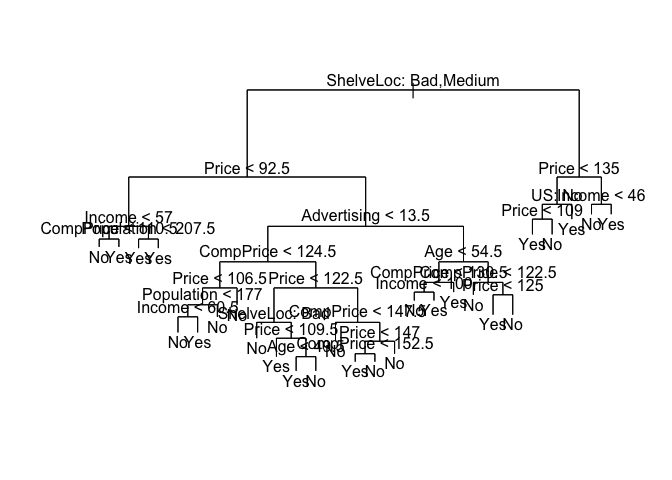
\includegraphics{Lab_Decision_Trees_files/figure-latex/unnamed-chunk-6-1.pdf}

The most important indicator of Sales appears to be shelving location,
since the first branch differentiates Good locations from Bad and Medium
locations

If we just type the name of the tree object, R prints output
corresponding to each branch of the tree. R displays the split criterion
(e.g.~Price\textless{}92.5), the number of observations in that branch,
the deviance, the overall prediction for the branch (Yes or No), and the
fraction of observations in that branch that take on values of Yes and
No. Branches that lead to terminal nodes are indicated using asterisks.

\begin{Shaded}
\begin{Highlighting}[]
\NormalTok{tree.carseats}
\end{Highlighting}
\end{Shaded}

\begin{verbatim}
## node), split, n, deviance, yval, (yprob)
##       * denotes terminal node
## 
##   1) root 400 541.500 No ( 0.59000 0.41000 )  
##     2) ShelveLoc: Bad,Medium 315 390.600 No ( 0.68889 0.31111 )  
##       4) Price < 92.5 46  56.530 Yes ( 0.30435 0.69565 )  
##         8) Income < 57 10  12.220 No ( 0.70000 0.30000 )  
##          16) CompPrice < 110.5 5   0.000 No ( 1.00000 0.00000 ) *
##          17) CompPrice > 110.5 5   6.730 Yes ( 0.40000 0.60000 ) *
##         9) Income > 57 36  35.470 Yes ( 0.19444 0.80556 )  
##          18) Population < 207.5 16  21.170 Yes ( 0.37500 0.62500 ) *
##          19) Population > 207.5 20   7.941 Yes ( 0.05000 0.95000 ) *
##       5) Price > 92.5 269 299.800 No ( 0.75465 0.24535 )  
##        10) Advertising < 13.5 224 213.200 No ( 0.81696 0.18304 )  
##          20) CompPrice < 124.5 96  44.890 No ( 0.93750 0.06250 )  
##            40) Price < 106.5 38  33.150 No ( 0.84211 0.15789 )  
##              80) Population < 177 12  16.300 No ( 0.58333 0.41667 )  
##               160) Income < 60.5 6   0.000 No ( 1.00000 0.00000 ) *
##               161) Income > 60.5 6   5.407 Yes ( 0.16667 0.83333 ) *
##              81) Population > 177 26   8.477 No ( 0.96154 0.03846 ) *
##            41) Price > 106.5 58   0.000 No ( 1.00000 0.00000 ) *
##          21) CompPrice > 124.5 128 150.200 No ( 0.72656 0.27344 )  
##            42) Price < 122.5 51  70.680 Yes ( 0.49020 0.50980 )  
##              84) ShelveLoc: Bad 11   6.702 No ( 0.90909 0.09091 ) *
##              85) ShelveLoc: Medium 40  52.930 Yes ( 0.37500 0.62500 )  
##               170) Price < 109.5 16   7.481 Yes ( 0.06250 0.93750 ) *
##               171) Price > 109.5 24  32.600 No ( 0.58333 0.41667 )  
##                 342) Age < 49.5 13  16.050 Yes ( 0.30769 0.69231 ) *
##                 343) Age > 49.5 11   6.702 No ( 0.90909 0.09091 ) *
##            43) Price > 122.5 77  55.540 No ( 0.88312 0.11688 )  
##              86) CompPrice < 147.5 58  17.400 No ( 0.96552 0.03448 ) *
##              87) CompPrice > 147.5 19  25.010 No ( 0.63158 0.36842 )  
##               174) Price < 147 12  16.300 Yes ( 0.41667 0.58333 )  
##                 348) CompPrice < 152.5 7   5.742 Yes ( 0.14286 0.85714 ) *
##                 349) CompPrice > 152.5 5   5.004 No ( 0.80000 0.20000 ) *
##               175) Price > 147 7   0.000 No ( 1.00000 0.00000 ) *
##        11) Advertising > 13.5 45  61.830 Yes ( 0.44444 0.55556 )  
##          22) Age < 54.5 25  25.020 Yes ( 0.20000 0.80000 )  
##            44) CompPrice < 130.5 14  18.250 Yes ( 0.35714 0.64286 )  
##              88) Income < 100 9  12.370 No ( 0.55556 0.44444 ) *
##              89) Income > 100 5   0.000 Yes ( 0.00000 1.00000 ) *
##            45) CompPrice > 130.5 11   0.000 Yes ( 0.00000 1.00000 ) *
##          23) Age > 54.5 20  22.490 No ( 0.75000 0.25000 )  
##            46) CompPrice < 122.5 10   0.000 No ( 1.00000 0.00000 ) *
##            47) CompPrice > 122.5 10  13.860 No ( 0.50000 0.50000 )  
##              94) Price < 125 5   0.000 Yes ( 0.00000 1.00000 ) *
##              95) Price > 125 5   0.000 No ( 1.00000 0.00000 ) *
##     3) ShelveLoc: Good 85  90.330 Yes ( 0.22353 0.77647 )  
##       6) Price < 135 68  49.260 Yes ( 0.11765 0.88235 )  
##        12) US: No 17  22.070 Yes ( 0.35294 0.64706 )  
##          24) Price < 109 8   0.000 Yes ( 0.00000 1.00000 ) *
##          25) Price > 109 9  11.460 No ( 0.66667 0.33333 ) *
##        13) US: Yes 51  16.880 Yes ( 0.03922 0.96078 ) *
##       7) Price > 135 17  22.070 No ( 0.64706 0.35294 )  
##        14) Income < 46 6   0.000 No ( 1.00000 0.00000 ) *
##        15) Income > 46 11  15.160 Yes ( 0.45455 0.54545 ) *
\end{verbatim}

In order to properly evaluate the performance of a classification tree
on these data, we must estimate the test error rather than simply
computing the training error. We split the observations into a training
set and a test set, build the tree using the training set, and evaluate
its performance on the test data. The predict() function can be used for
this purpose. In the case of a classification tree, the argument
type=``class'' instructs R to return the actual class prediction. This
approach leads to correct predictions for around 71.5 \% of the
locations in the test data set.

\begin{Shaded}
\begin{Highlighting}[]
\KeywordTok{set.seed}\NormalTok{(}\DecValTok{2}\NormalTok{)}
\NormalTok{train =}\StringTok{ }\KeywordTok{sample}\NormalTok{(}\DecValTok{1}\OperatorTok{:}\KeywordTok{nrow}\NormalTok{(Carseats), }\DecValTok{200}\NormalTok{)}
\NormalTok{Carseats.test =}\StringTok{ }\NormalTok{Carseats[}\OperatorTok{-}\NormalTok{train,]}
\NormalTok{High.test =}\StringTok{ }\NormalTok{High[}\OperatorTok{-}\NormalTok{train]}

\NormalTok{tree.carseats =}\StringTok{ }\KeywordTok{tree}\NormalTok{(High }\OperatorTok{~}\StringTok{ }\NormalTok{.}\OperatorTok{-}\NormalTok{Sales, Carseats, }\DataTypeTok{subset =}\NormalTok{ train)}

\NormalTok{tree.pred =}\StringTok{ }\KeywordTok{predict}\NormalTok{(tree.carseats, Carseats.test, }\DataTypeTok{type =} \StringTok{"class"}\NormalTok{)}
\KeywordTok{table}\NormalTok{(tree.pred, High.test)}
\end{Highlighting}
\end{Shaded}

\begin{verbatim}
##          High.test
## tree.pred No Yes
##       No  86  27
##       Yes 30  57
\end{verbatim}

\begin{Shaded}
\begin{Highlighting}[]
\NormalTok{(}\DecValTok{86} \OperatorTok{+}\StringTok{ }\DecValTok{57}\NormalTok{)}\OperatorTok{/}\DecValTok{200} 
\end{Highlighting}
\end{Shaded}

\begin{verbatim}
## [1] 0.715
\end{verbatim}

Next, we consider whether pruning the tree might lead to improved
results. The function cv.tree() performs cross validation in order to
determine the optimal level of tree complexity; cost complexity pruning
is used in order to select a sequence of trees for consideration.

We use the argument FUN=prune.misclass in order to indicate that we want
the classification error rate to guide the cross validation and pruning
process, rather than the default for the cv.tree() function, which is
deviance.

The cv.tree() function reports the number of terminal nodes of each tree
considered (size) as well as the corresponding error rate and the value
of the cost complexity parameter used (k corresponds to alpha).

\begin{Shaded}
\begin{Highlighting}[]
\KeywordTok{set.seed}\NormalTok{(}\DecValTok{3}\NormalTok{)}
\NormalTok{cv.carseats =}\StringTok{ }\KeywordTok{cv.tree}\NormalTok{(tree.carseats, }\DataTypeTok{FUN =}\NormalTok{ prune.misclass)}

\KeywordTok{names}\NormalTok{(cv.carseats)}
\end{Highlighting}
\end{Shaded}

\begin{verbatim}
## [1] "size"   "dev"    "k"      "method"
\end{verbatim}

\begin{Shaded}
\begin{Highlighting}[]
\NormalTok{cv.carseats}\OperatorTok{$}\NormalTok{size}
\end{Highlighting}
\end{Shaded}

\begin{verbatim}
## [1] 19 17 14 13  9  7  3  2  1
\end{verbatim}

\begin{Shaded}
\begin{Highlighting}[]
\NormalTok{cv.carseats}\OperatorTok{$}\NormalTok{dev}
\end{Highlighting}
\end{Shaded}

\begin{verbatim}
## [1] 55 55 53 52 50 56 69 65 80
\end{verbatim}

\begin{Shaded}
\begin{Highlighting}[]
\NormalTok{cv.carseats}\OperatorTok{$}\NormalTok{k}
\end{Highlighting}
\end{Shaded}

\begin{verbatim}
## [1]       -Inf  0.0000000  0.6666667  1.0000000  1.7500000  2.0000000
## [7]  4.2500000  5.0000000 23.0000000
\end{verbatim}

\begin{Shaded}
\begin{Highlighting}[]
\NormalTok{cv.carseats}\OperatorTok{$}\NormalTok{method}
\end{Highlighting}
\end{Shaded}

\begin{verbatim}
## [1] "misclass"
\end{verbatim}

Note that, despite the name, dev corresponds to the cross validation
error rate in this instance. The tree with 9 terminal nodes results in
the lowest cross validation error rate, with 50 cross validation errors.
We plot the error rate as a function of both size and k.

\begin{Shaded}
\begin{Highlighting}[]
\KeywordTok{par}\NormalTok{(}\DataTypeTok{mfrow =} \KeywordTok{c}\NormalTok{(}\DecValTok{1}\NormalTok{, }\DecValTok{2}\NormalTok{))}
\KeywordTok{plot}\NormalTok{(cv.carseats}\OperatorTok{$}\NormalTok{size, cv.carseats}\OperatorTok{$}\NormalTok{dev, }\DataTypeTok{type =} \StringTok{"b"}\NormalTok{)}
\KeywordTok{plot}\NormalTok{(cv.carseats}\OperatorTok{$}\NormalTok{k, cv.carseats}\OperatorTok{$}\NormalTok{dev, }\DataTypeTok{type =} \StringTok{"b"}\NormalTok{)}
\end{Highlighting}
\end{Shaded}

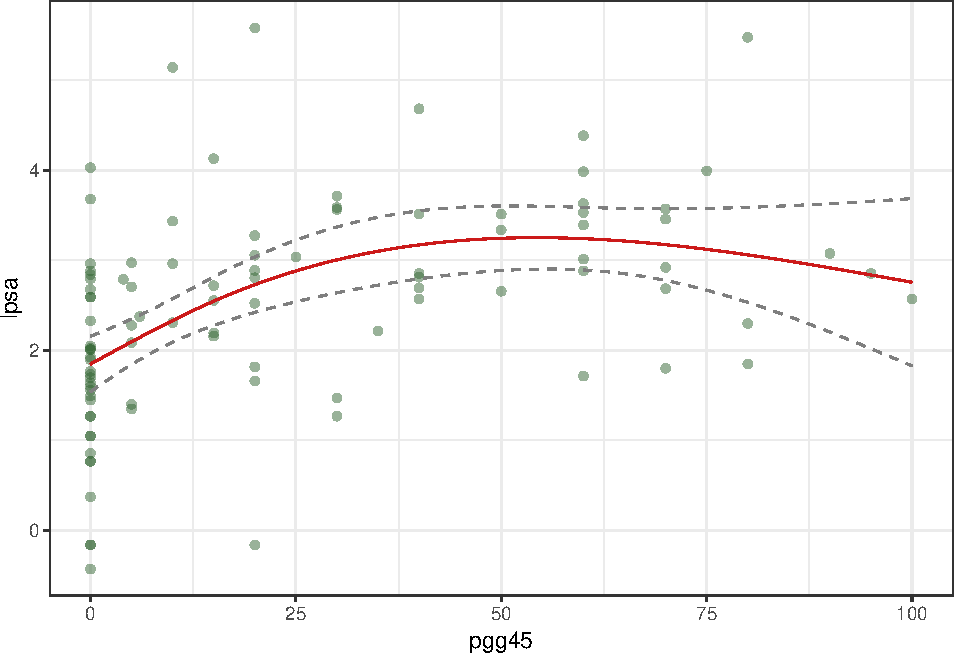
\includegraphics{Lab_Decision_Trees_files/figure-latex/unnamed-chunk-10-1.pdf}

We now apply the prune.misclass() function in order to prune the tree to
obtain the nine node tree

\begin{Shaded}
\begin{Highlighting}[]
\NormalTok{prune.carseats =}\StringTok{ }\KeywordTok{prune.misclass}\NormalTok{(tree.carseats, }\DataTypeTok{best =} \DecValTok{9}\NormalTok{)}
\KeywordTok{plot}\NormalTok{(prune.carseats)}
\KeywordTok{text}\NormalTok{(prune.carseats, }\DataTypeTok{pretty =} \DecValTok{0}\NormalTok{)}
\end{Highlighting}
\end{Shaded}

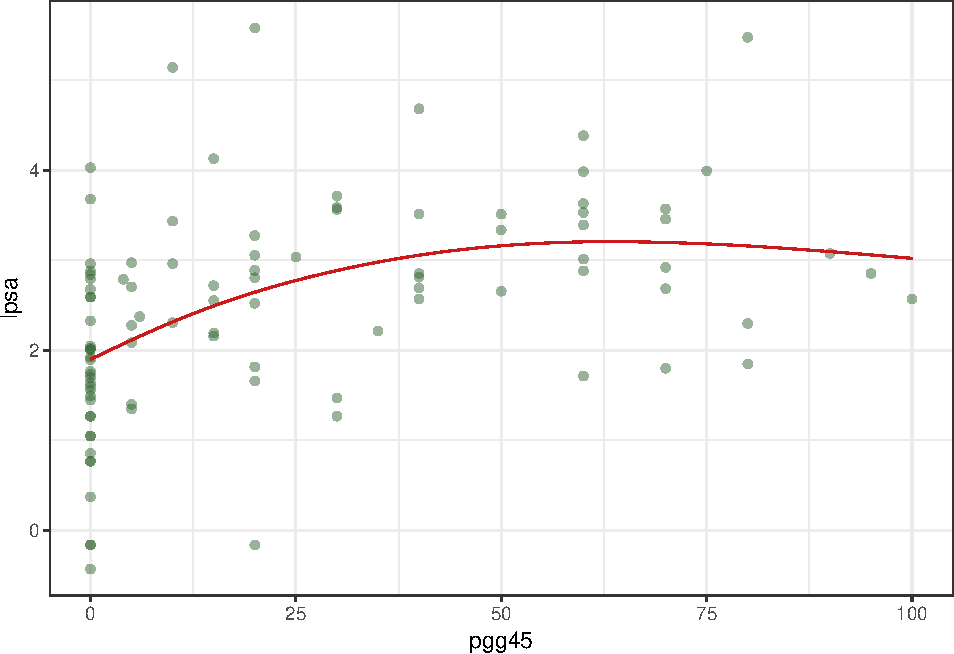
\includegraphics{Lab_Decision_Trees_files/figure-latex/unnamed-chunk-11-1.pdf}

we apply the predict() function to see how well does this pruned tree
perform on the test data set.

\begin{Shaded}
\begin{Highlighting}[]
\NormalTok{tree.pred =}\StringTok{ }\KeywordTok{predict}\NormalTok{(prune.carseats, Carseats.test, }\DataTypeTok{type =} \StringTok{"class"}\NormalTok{)}
\KeywordTok{table}\NormalTok{(tree.pred, High.test)}
\end{Highlighting}
\end{Shaded}

\begin{verbatim}
##          High.test
## tree.pred No Yes
##       No  94  24
##       Yes 22  60
\end{verbatim}

\begin{Shaded}
\begin{Highlighting}[]
\NormalTok{(}\DecValTok{94} \OperatorTok{+}\StringTok{ }\DecValTok{60}\NormalTok{)}\OperatorTok{/}\DecValTok{200}
\end{Highlighting}
\end{Shaded}

\begin{verbatim}
## [1] 0.77
\end{verbatim}

Now 77 \% of the test observations are correctly classified, so not only
has the pruning process produced a more interpretable tree, but it has
also improved the classification accuracy. If we increase the value of
best, we obtain a larger pruned tree with lower classification accuracy

\begin{Shaded}
\begin{Highlighting}[]
\NormalTok{prune.carseats =}\StringTok{ }\KeywordTok{prune.misclass}\NormalTok{(tree.carseats, }\DataTypeTok{best=}\DecValTok{15}\NormalTok{)}
\KeywordTok{plot}\NormalTok{(prune.carseats)}
\KeywordTok{text}\NormalTok{(prune.carseats, }\DataTypeTok{pretty =} \DecValTok{0}\NormalTok{)}
\end{Highlighting}
\end{Shaded}

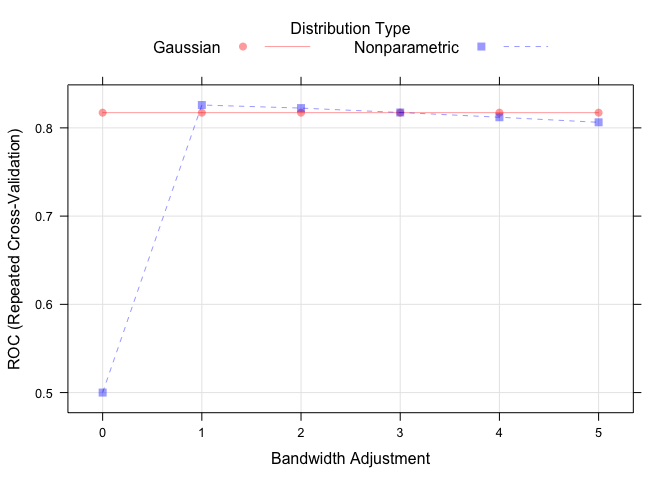
\includegraphics{Lab_Decision_Trees_files/figure-latex/unnamed-chunk-13-1.pdf}

\begin{Shaded}
\begin{Highlighting}[]
\NormalTok{tree.pred =}\StringTok{ }\KeywordTok{predict}\NormalTok{(prune.carseats, Carseats.test, }\DataTypeTok{type =} \StringTok{"class"}\NormalTok{)}
\KeywordTok{table}\NormalTok{(tree.pred, High.test)}
\end{Highlighting}
\end{Shaded}

\begin{verbatim}
##          High.test
## tree.pred No Yes
##       No  86  22
##       Yes 30  62
\end{verbatim}

\begin{Shaded}
\begin{Highlighting}[]
\NormalTok{(}\DecValTok{86} \OperatorTok{+}\StringTok{ }\DecValTok{62}\NormalTok{)}\OperatorTok{/}\DecValTok{200}
\end{Highlighting}
\end{Shaded}

\begin{verbatim}
## [1] 0.74
\end{verbatim}

\section{Fitting Regression Trees}\label{fitting-regression-trees}

Here we fit a regression tree to the Boston data set. First, we create a
training set, and fit the tree to the training data.

\begin{Shaded}
\begin{Highlighting}[]
\KeywordTok{library}\NormalTok{(MASS)}
\KeywordTok{set.seed}\NormalTok{(}\DecValTok{1}\NormalTok{)}
\NormalTok{train =}\StringTok{ }\KeywordTok{sample}\NormalTok{(}\DecValTok{1}\OperatorTok{:}\KeywordTok{nrow}\NormalTok{(Boston), }\KeywordTok{nrow}\NormalTok{(Boston)}\OperatorTok{/}\DecValTok{2}\NormalTok{)}

\NormalTok{tree.boston =}\StringTok{ }\KeywordTok{tree}\NormalTok{(medv }\OperatorTok{~}\StringTok{ }\NormalTok{. , Boston, }\DataTypeTok{subset =}\NormalTok{ train)}
\KeywordTok{summary}\NormalTok{(tree.boston)}
\end{Highlighting}
\end{Shaded}

\begin{verbatim}
## 
## Regression tree:
## tree(formula = medv ~ ., data = Boston, subset = train)
## Variables actually used in tree construction:
## [1] "lstat" "rm"    "dis"  
## Number of terminal nodes:  8 
## Residual mean deviance:  12.65 = 3099 / 245 
## Distribution of residuals:
##      Min.   1st Qu.    Median      Mean   3rd Qu.      Max. 
## -14.10000  -2.04200  -0.05357   0.00000   1.96000  12.60000
\end{verbatim}

Notice that the output of summary() indicates that only three of the
variables have been used in constructing the tree. In the context of a
regression tree, the deviance is simply the sum of squared errors for
the tree. We now plot the tree

\begin{Shaded}
\begin{Highlighting}[]
\KeywordTok{plot}\NormalTok{(tree.boston)}
\KeywordTok{text}\NormalTok{(tree.boston, }\DataTypeTok{pretty =} \DecValTok{0}\NormalTok{)}
\end{Highlighting}
\end{Shaded}

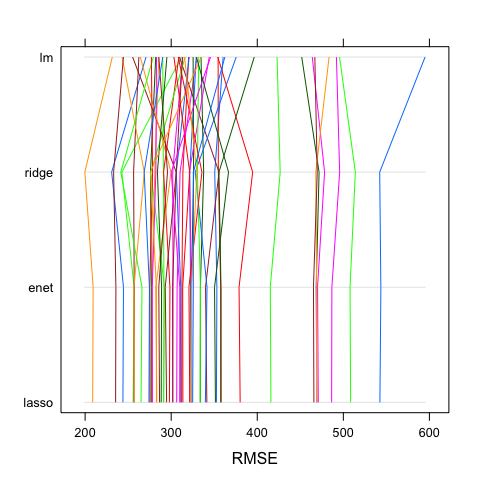
\includegraphics{Lab_Decision_Trees_files/figure-latex/unnamed-chunk-15-1.pdf}

The variable lstat measures the percentage of individuals with lower
socioeconomic status. The tree indicates that lower values of lstat
correspond to more expensive houses. The tree predicts a median house
price of \$46, 400 for larger homes in suburbs in which residents have
high socioeconomic status (rm\textgreater{}=7.437 and
lstat\textless{}9.715).

Now we use the cv.tree() function to see whether pruning the tree will
improve performance.

\begin{Shaded}
\begin{Highlighting}[]
\NormalTok{cv.boston =}\StringTok{ }\KeywordTok{cv.tree}\NormalTok{(tree.boston)}

\KeywordTok{plot}\NormalTok{(cv.boston}\OperatorTok{$}\NormalTok{size, cv.boston}\OperatorTok{$}\NormalTok{dev, }\DataTypeTok{type =} \StringTok{'b'}\NormalTok{)}
\end{Highlighting}
\end{Shaded}

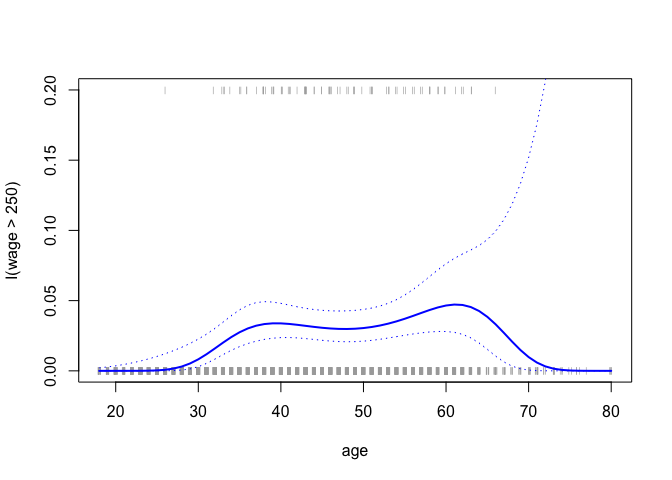
\includegraphics{Lab_Decision_Trees_files/figure-latex/unnamed-chunk-16-1.pdf}

In this case, the most complex tree is selected by cross validation.
However, if we wish to prune the tree, we could do so as follows, using
the prune.tree() function

\begin{Shaded}
\begin{Highlighting}[]
\NormalTok{prune.boston=}\KeywordTok{prune.tree}\NormalTok{(tree.boston, }\DataTypeTok{best =} \DecValTok{5}\NormalTok{)}
\KeywordTok{plot}\NormalTok{(prune.boston)}
\KeywordTok{text}\NormalTok{(prune.boston, }\DataTypeTok{pretty =} \DecValTok{0}\NormalTok{)}
\end{Highlighting}
\end{Shaded}

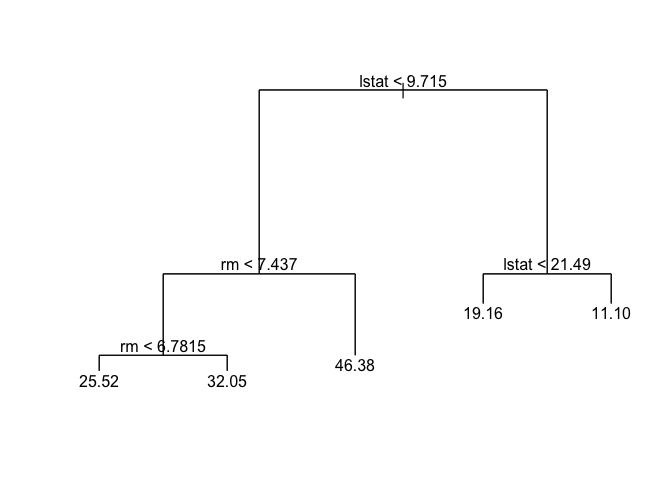
\includegraphics{Lab_Decision_Trees_files/figure-latex/unnamed-chunk-17-1.pdf}

In keeping with the cross validation results, we use the unpruned tree
to make predictions on the test set.

\begin{Shaded}
\begin{Highlighting}[]
\NormalTok{yhat =}\StringTok{ }\KeywordTok{predict}\NormalTok{(tree.boston, }\DataTypeTok{newdata =}\NormalTok{ Boston[}\OperatorTok{-}\NormalTok{train ,])}
\NormalTok{boston.test =}\StringTok{ }\NormalTok{Boston[}\OperatorTok{-}\NormalTok{train, }\StringTok{"medv"}\NormalTok{]}

\KeywordTok{plot}\NormalTok{(yhat, boston.test)}
\KeywordTok{abline}\NormalTok{(}\DecValTok{0}\NormalTok{,}\DecValTok{1}\NormalTok{)}
\end{Highlighting}
\end{Shaded}

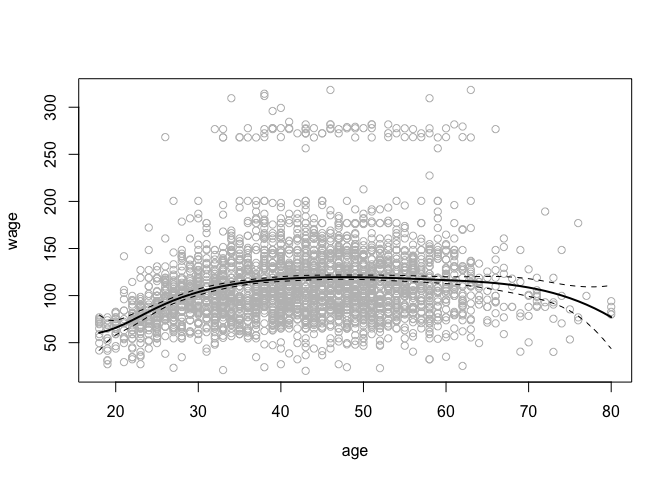
\includegraphics{Lab_Decision_Trees_files/figure-latex/unnamed-chunk-18-1.pdf}

\begin{Shaded}
\begin{Highlighting}[]
\KeywordTok{mean}\NormalTok{((yhat }\OperatorTok{-}\StringTok{ }\NormalTok{boston.test)}\OperatorTok{^}\DecValTok{2}\NormalTok{)}
\end{Highlighting}
\end{Shaded}

\begin{verbatim}
## [1] 25.04559
\end{verbatim}

In other words, the test set MSE associated with the regression tree is
25.05. The square root of the MSE is therefore around 5.005, indicating
that this model leads to test predictions that are within around \$5,
005 of the true median home value for the suburb.

\section{Bagging and Random Forests}\label{bagging-and-random-forests}

Here we apply bagging and random forests to the Boston data, using the
randomForest package. Bagging is simply a special case of a random
forest with m = p.~Therefore, the randomForest() function can be used to
perform both random forests and bagging. We perform bagging as follows

\begin{Shaded}
\begin{Highlighting}[]
\KeywordTok{library}\NormalTok{(randomForest)}
\end{Highlighting}
\end{Shaded}

\begin{verbatim}
## randomForest 4.6-14
\end{verbatim}

\begin{verbatim}
## Type rfNews() to see new features/changes/bug fixes.
\end{verbatim}

\begin{Shaded}
\begin{Highlighting}[]
\KeywordTok{set.seed}\NormalTok{ (}\DecValTok{1}\NormalTok{)}

\NormalTok{bag.boston =}\StringTok{ }\KeywordTok{randomForest}\NormalTok{(medv }\OperatorTok{~}\StringTok{ }\NormalTok{., }\DataTypeTok{data =}\NormalTok{ Boston, }\DataTypeTok{subset =}\NormalTok{ train,}
                          \DataTypeTok{mtry =} \DecValTok{13}\NormalTok{,}
                          \DataTypeTok{importance =} \OtherTok{TRUE}\NormalTok{)}
\NormalTok{bag.boston}
\end{Highlighting}
\end{Shaded}

\begin{verbatim}
## 
## Call:
##  randomForest(formula = medv ~ ., data = Boston, mtry = 13, importance = TRUE,      subset = train) 
##                Type of random forest: regression
##                      Number of trees: 500
## No. of variables tried at each split: 13
## 
##           Mean of squared residuals: 11.15723
##                     % Var explained: 86.49
\end{verbatim}

The argument mtry=13 indicates that all 13 predictors should be
considered for each split of the tree---in other words, that bagging
should be done. How well does this bagged model perform on the test set?

\begin{Shaded}
\begin{Highlighting}[]
\NormalTok{yhat.bag =}\StringTok{ }\KeywordTok{predict}\NormalTok{(bag.boston, }\DataTypeTok{newdata =}\NormalTok{ Boston[}\OperatorTok{-}\NormalTok{train,])}

\KeywordTok{plot}\NormalTok{(yhat.bag, boston.test)}
\KeywordTok{abline}\NormalTok{(}\DecValTok{0}\NormalTok{,}\DecValTok{1}\NormalTok{)}
\end{Highlighting}
\end{Shaded}

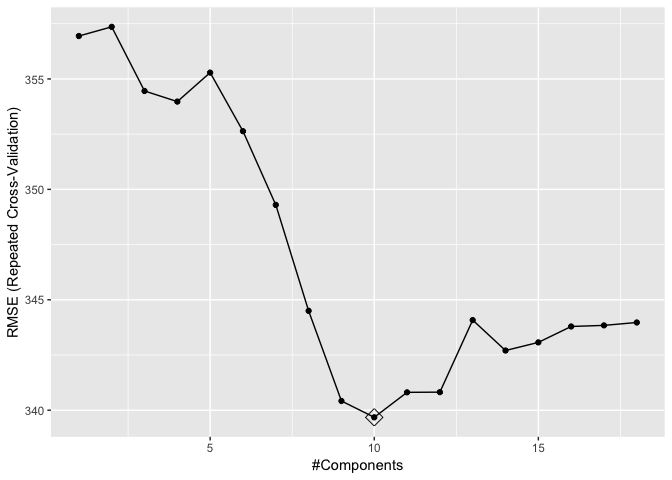
\includegraphics{Lab_Decision_Trees_files/figure-latex/unnamed-chunk-20-1.pdf}

\begin{Shaded}
\begin{Highlighting}[]
\KeywordTok{mean}\NormalTok{((yhat.bag }\OperatorTok{-}\StringTok{ }\NormalTok{boston.test)}\OperatorTok{^}\DecValTok{2}\NormalTok{)}
\end{Highlighting}
\end{Shaded}

\begin{verbatim}
## [1] 13.50808
\end{verbatim}

The test set MSE associated with the bagged regression tree is 13.5,
almost half that obtained using an optimally pruned single tree. We
could change the number of trees grown by randomForest() using the ntree
argument.

\begin{Shaded}
\begin{Highlighting}[]
\NormalTok{bag.boston=}\KeywordTok{randomForest}\NormalTok{(medv }\OperatorTok{~}\StringTok{ }\NormalTok{., }\DataTypeTok{data =}\NormalTok{ Boston, }\DataTypeTok{subset =}\NormalTok{ train, }
                        \DataTypeTok{mtry =} \DecValTok{13}\NormalTok{, }
                        \DataTypeTok{ntree =} \DecValTok{25}\NormalTok{)}

\NormalTok{yhat.bag =}\StringTok{ }\KeywordTok{predict}\NormalTok{(bag.boston, }\DataTypeTok{newdata =}\NormalTok{ Boston[}\OperatorTok{-}\NormalTok{train,])}

\KeywordTok{mean}\NormalTok{((yhat.bag }\OperatorTok{-}\StringTok{ }\NormalTok{boston.test)}\OperatorTok{^}\DecValTok{2}\NormalTok{) }
\end{Highlighting}
\end{Shaded}

\begin{verbatim}
## [1] 13.94835
\end{verbatim}

Growing a random forest proceeds in exactly the same way, except that we
use a smaller value of the mtry argument. By default, randomForest()
uses p/3 variables when building a random forest of regression trees,
and √p variables when building a random forest of classification trees.
Here we use mtry = 6.

\begin{Shaded}
\begin{Highlighting}[]
\KeywordTok{set.seed}\NormalTok{(}\DecValTok{1}\NormalTok{)}
\NormalTok{rf.boston =}\StringTok{ }\KeywordTok{randomForest}\NormalTok{(medv }\OperatorTok{~}\StringTok{ }\NormalTok{., }\DataTypeTok{data =}\NormalTok{ Boston, }\DataTypeTok{subset =}\NormalTok{ train,}
                       \DataTypeTok{mtry =} \DecValTok{6}\NormalTok{,}
                       \DataTypeTok{importance =} \OtherTok{TRUE}\NormalTok{)}

\NormalTok{yhat.rf =}\StringTok{ }\KeywordTok{predict}\NormalTok{(rf.boston, }\DataTypeTok{newdata =}\NormalTok{ Boston[}\OperatorTok{-}\NormalTok{train ,])}
\KeywordTok{mean}\NormalTok{((yhat.rf }\OperatorTok{-}\StringTok{ }\NormalTok{boston.test)}\OperatorTok{^}\DecValTok{2}\NormalTok{)}
\end{Highlighting}
\end{Shaded}

\begin{verbatim}
## [1] 11.66454
\end{verbatim}

The test set MSE is 11.66; this indicates that random forests yielded an
improvement over bagging in this case.

Using the importance() function, we can view the importance of each
variable.

\begin{Shaded}
\begin{Highlighting}[]
\KeywordTok{importance}\NormalTok{(rf.boston)}
\end{Highlighting}
\end{Shaded}

\begin{verbatim}
##           %IncMSE IncNodePurity
## crim    12.132320     986.50338
## zn       1.955579      57.96945
## indus    9.069302     882.78261
## chas     2.210835      45.22941
## nox     11.104823    1044.33776
## rm      31.784033    6359.31971
## age     10.962684     516.82969
## dis     15.015236    1224.11605
## rad      4.118011      95.94586
## tax      8.587932     502.96719
## ptratio 12.503896     830.77523
## black    6.702609     341.30361
## lstat   30.695224    7505.73936
\end{verbatim}

Two measures of variable importance are reported. The former is based
upon the mean decrease of accuracy in predictions on the out of bag
samples when a given variable is excluded from the model. The latter is
a measure of the total decrease in node impurity that results from
splits over that variable, averaged over all trees.

In the case of regression trees, the node impurity is measured by the
training RSS, and for classification trees by the deviance. Plots of
these importance measures can be produced using the varImpPlot()
function.

\begin{Shaded}
\begin{Highlighting}[]
\KeywordTok{varImpPlot}\NormalTok{(rf.boston)}
\end{Highlighting}
\end{Shaded}

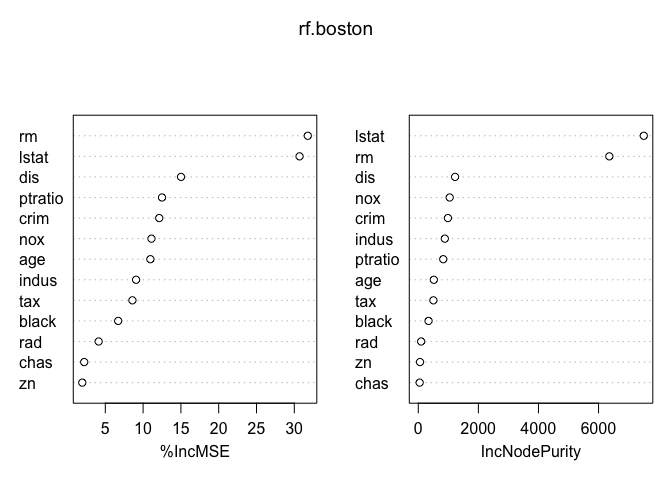
\includegraphics{Lab_Decision_Trees_files/figure-latex/unnamed-chunk-24-1.pdf}

The results indicate that across all of the trees considered in the
random forest, the wealth level of the community (lstat) and the house
size (rm) are by far the two most important variables.

\section{Boosting}\label{boosting}

Here we use the gbm package, and within it the gbm() function, to fit
boosted regression trees to the Boston data set. We run gbm() with the
option distribution=``gaussian'' since this is a regression problem; if
it were a binary classification problem, we would use
distribution=``bernoulli''. The argument n.trees=5000 indicates that we
want 5000 trees, and the option interaction.depth=4 limits the depth of
each tree.

\begin{Shaded}
\begin{Highlighting}[]
\KeywordTok{library}\NormalTok{(gbm)}
\end{Highlighting}
\end{Shaded}

\begin{verbatim}
## Loaded gbm 2.1.5
\end{verbatim}

\begin{Shaded}
\begin{Highlighting}[]
\KeywordTok{set.seed}\NormalTok{(}\DecValTok{1}\NormalTok{)}
\NormalTok{boost.boston =}\StringTok{ }\KeywordTok{gbm}\NormalTok{(medv }\OperatorTok{~}\StringTok{ }\NormalTok{., }\DataTypeTok{data =}\NormalTok{ Boston[train,],}
                 \DataTypeTok{distribution =} \StringTok{"gaussian"}\NormalTok{,}
                 \DataTypeTok{n.trees =} \DecValTok{5000}\NormalTok{, }
                 \DataTypeTok{interaction.depth =} \DecValTok{4}\NormalTok{)}
\end{Highlighting}
\end{Shaded}

The summary() function produces a relative influence plot and also
outputs the relative influence statistics.

\begin{Shaded}
\begin{Highlighting}[]
\KeywordTok{summary}\NormalTok{(boost.boston)}
\end{Highlighting}
\end{Shaded}

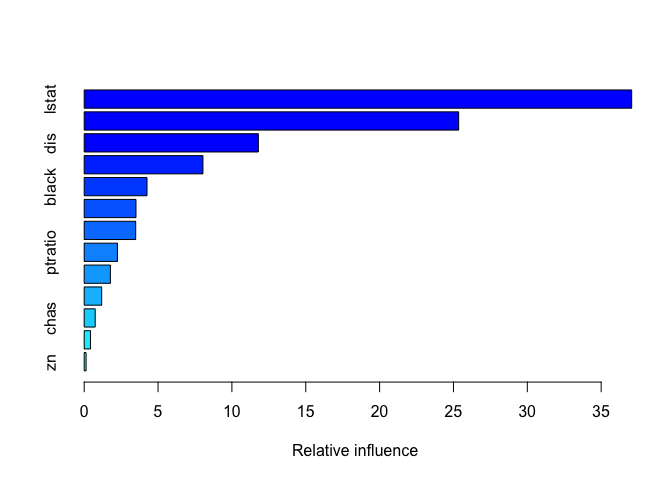
\includegraphics{Lab_Decision_Trees_files/figure-latex/unnamed-chunk-26-1.pdf}

\begin{verbatim}
##             var    rel.inf
## lstat     lstat 37.0661275
## rm           rm 25.3533123
## dis         dis 11.7903016
## crim       crim  8.0388750
## black     black  4.2531659
## nox         nox  3.5058570
## age         age  3.4868724
## ptratio ptratio  2.2500385
## indus     indus  1.7725070
## tax         tax  1.1836592
## chas       chas  0.7441319
## rad         rad  0.4274311
## zn           zn  0.1277206
\end{verbatim}

We see that lstat and rm are by far the most important variables. We can
also produce partial dependence plots for these two variables. These
plots illustrate the marginal effect of the selected variables on the
response after integrating out the other variables. In this case, as we
might expect, median house prices are increasing with rm and decreasing
with lstat.

\begin{Shaded}
\begin{Highlighting}[]
\KeywordTok{par}\NormalTok{(}\DataTypeTok{mfrow =} \KeywordTok{c}\NormalTok{(}\DecValTok{1}\NormalTok{, }\DecValTok{2}\NormalTok{)) }
\KeywordTok{plot}\NormalTok{(boost.boston, }\DataTypeTok{i =} \StringTok{"rm"}\NormalTok{) }
\end{Highlighting}
\end{Shaded}

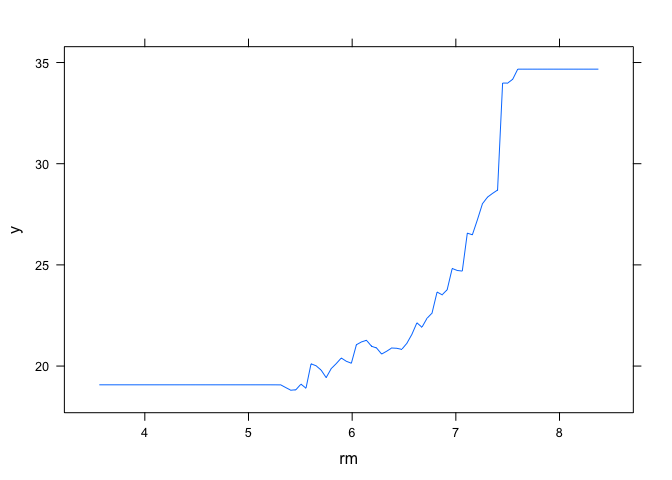
\includegraphics{Lab_Decision_Trees_files/figure-latex/unnamed-chunk-27-1.pdf}

\begin{Shaded}
\begin{Highlighting}[]
\KeywordTok{plot}\NormalTok{(boost.boston, }\DataTypeTok{i =} \StringTok{"lstat"}\NormalTok{)}
\end{Highlighting}
\end{Shaded}

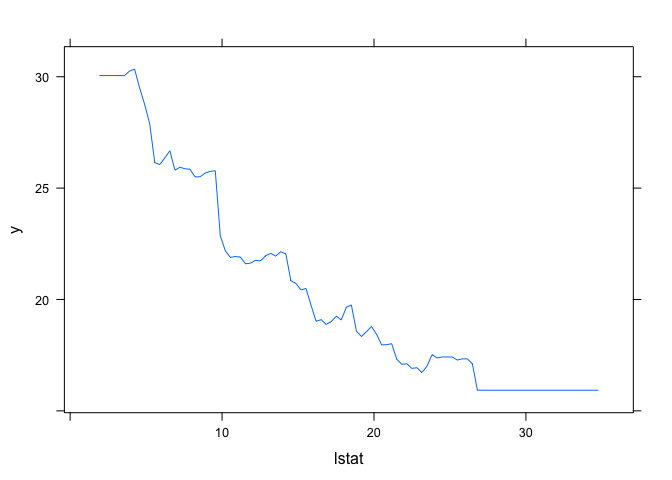
\includegraphics{Lab_Decision_Trees_files/figure-latex/unnamed-chunk-27-2.pdf}

We now use the boosted model to predict medv on the test set

\begin{Shaded}
\begin{Highlighting}[]
\NormalTok{yhat.boost =}\StringTok{ }\KeywordTok{predict}\NormalTok{(boost.boston, }\DataTypeTok{newdata =}\NormalTok{ Boston[}\OperatorTok{-}\NormalTok{train,], }
                   \DataTypeTok{n.trees =} \DecValTok{5000}\NormalTok{)}

\KeywordTok{mean}\NormalTok{((yhat.boost }\OperatorTok{-}\StringTok{ }\NormalTok{boston.test)}\OperatorTok{^}\DecValTok{2}\NormalTok{)}
\end{Highlighting}
\end{Shaded}

\begin{verbatim}
## [1] 10.81479
\end{verbatim}

The test MSE obtained is 10.8; superior to the test MSE for random
forests and to that for bagging. If we want to, we can perform boosting
with a different value of the shrinkage parameter λ. The default value
is 0.001, but this is easily modified. Here we take λ = 0.2.

\begin{Shaded}
\begin{Highlighting}[]
\NormalTok{boost.boston =}\StringTok{ }\KeywordTok{gbm}\NormalTok{(medv }\OperatorTok{~}\StringTok{ }\NormalTok{., }\DataTypeTok{data =}\NormalTok{ Boston[train,],}
                 \DataTypeTok{distribution =} \StringTok{"gaussian"}\NormalTok{,}
                 \DataTypeTok{n.trees =} \DecValTok{5000}\NormalTok{, }\DataTypeTok{interaction.depth =} \DecValTok{4}\NormalTok{,}
                 \DataTypeTok{shrinkage =} \FloatTok{0.2}\NormalTok{, }
                 \DataTypeTok{verbose =}\NormalTok{ F)}

\NormalTok{yhat.boost =}\StringTok{ }\KeywordTok{predict}\NormalTok{(boost.boston, }\DataTypeTok{newdata =}\NormalTok{ Boston[}\OperatorTok{-}\NormalTok{train,], }
                     \DataTypeTok{n.trees =} \DecValTok{5000}\NormalTok{)}

\KeywordTok{mean}\NormalTok{((yhat.boost }\OperatorTok{-}\StringTok{ }\NormalTok{boston.test)}\OperatorTok{^}\DecValTok{2}\NormalTok{)}
\end{Highlighting}
\end{Shaded}

\begin{verbatim}
## [1] 11.51109
\end{verbatim}

In this case, using = 0.2 leads to a higher test MSE than = 0.001.


\end{document}
